\setcounter{section}{34}
\section{Куча Фибоначчи: реализация merge, insert, getMin и extractMin.}
\par \textbf{Определение:} \textit{Куча Фибоначчи} - набор деревьев, удовлетворяющих свойствам кучи. Корни всех деревьев хранятся в списке.
\subsection*{Реализация операций:} \begin{enumerate}
    \item getMin - при всех операциях поддерживаем указатель на минимальный корень. Асимптотика: $O(1)$.
    \item merge - связываем указатель на последнее дерево одного списка с указателем на первое дерево другого списка (просто склеиваем два списка). Новый минимум выбираем из двух значений минимумов объединяемых куч. Асимптотика: $O(1)$.
    \item insert - создаём кучу из одного этого элемента и делаем merge. Асимптотика: $O(1)$.
    \item extractMin - удаляем минимальный корень, всех его детей добавляем в список корней и применяем consolidate ("причесываем" кучу). Асимптотика: $O(\log n)^*$.
    \lstinputlisting[language=C++,
emph={int,char,double,float,unsigned},
emphstyle={\color{blue}}
]{code/35-39_consolidate.cpp}
\par \textbf{Обоснование асимптотики:} Поддерживаем на каждом корне по одной монетке. В extractMin кладем не больше $D(n)$ монеток. Время работы consolidate=$\#$cнятых монеток $\Rightarrow$ учётное время работы extractMin=$\#$положенных монеток $+$ время работы $-$ $\#$снятых монеток (при объединении двух деревьев снимаем с одного из корней монетку). Количество снятых монеток равно времени работы consolidate (время переноса детей в список $\leqslant D(n)$), а количество положенных монеток $\leqslant D(n)$. Таким образом, получаем асимптотику $O(D(n))^*$ (позже докажем, что это то же самое, что $O(\log n)^*$)
\end{enumerate}

\setcounter{section}{35}
\section{Куча Фибоначчи: реализация decreaseKey, амортизированное время работы.}
\par Уменьшаем нужный элемент $x$. Если неравенство с его родителем $y$ нарушилось (он стал меньше), то переносим его в список корней.
\begin{enumerate}
    \item Если y.mark == false, то меняем его значение на true
    \item Если y.mark == true, то выносим все это поддерево в список корней и ставим y.mark=false. Повторяем эти же действия для родителя $y$
\end{enumerate}
\lstinputlisting[language=C++,
emph={int,char,double,float,unsigned},
emphstyle={\color{blue}}
]{code/35-39_decrease.cpp}
\par \textbf{Обоснование асимптотики:} На каждую вершину с mark==true кладём по 2 монетки. Тогда
\begin{enumerate}
    \item Если y.mark == false, то асимптотика O(1)
    \item Если y.mark == true, то одной монеткой с $y$ расплачиваемся за перенос и одну оставляем на $y$ как на новом корне.
\end{enumerate}
\par Таким образом, получаем асимптотику $O(1)^*$.

\setcounter{section}{36}
\section{Куча Фибоначчи: оценка на максимальную степень корня $D(n)$ в куче на $n$ вершинах.}
\par $D(n)=\max \{k \; | \; S(k) \leqslant n\}$, так как при $S(k)>n$ ответ нам уже не подойдет, ибо если минимальное количество вершин в дереве с такой степенью корня $>n$, то ровно $n$ вершин там никак не может быть (про $S(k)$ см. билет 38). Так как $S(k)=\Omega(\varphi^k)$ (см. билет 38-39), то $D(n)=k_{\max} =O(\log_\varphi n)=O(\log n)$


\setcounter{section}{37}
\section{Куча Фибоначчи: минимальное количество вершин $S(k)$ в дереве с корнем степени k.}
\par Пронумеруем детей в порядке их подвешивания к этому корню ($u_0, \ldots, u_{k-1}$). Тогда в момент когда $u_i$ подвешивали к корню у него была степень хотя бы $i$ (из-за предыдущих $u_i$, так как мы объединяем деревья с одинаковой степенью). Сейчас у вершины $u_i$ степень $\geqslant i-1$, так как мы могли отрезать от нее не более одного сына в результате decreaseKey.
\begin{figure}[h]
    \centering
    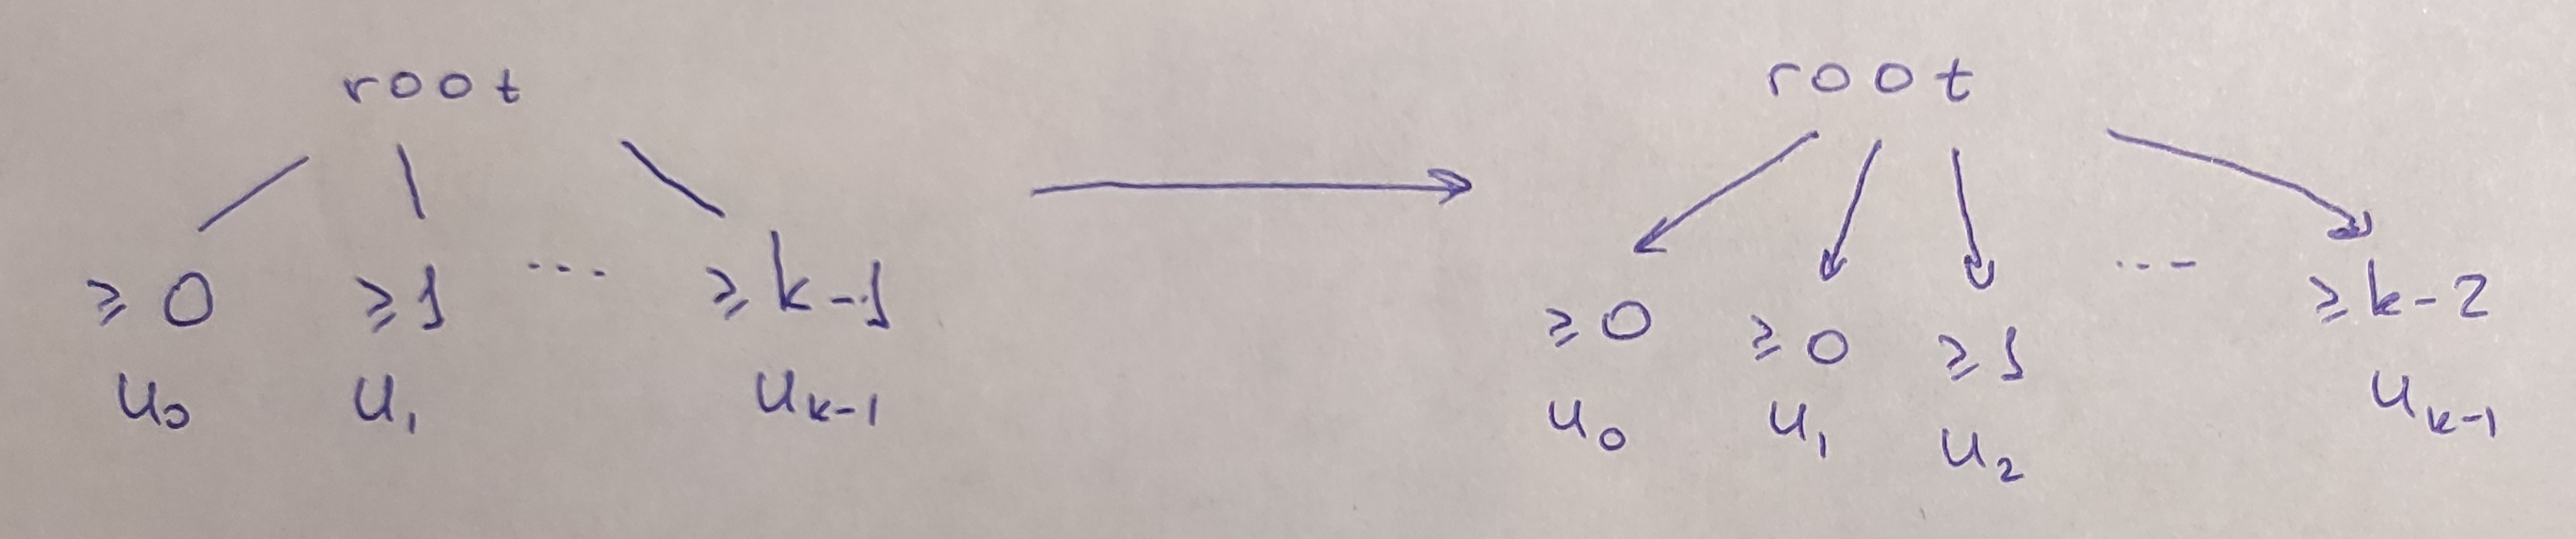
\includegraphics[width=\linewidth]{images/38}
\end{figure}
\par Таким образом получаем следующее неравенство для $S$: 
$$S(k) \geqslant 2 + \sum\limits_{i=0}^{k-2} S(i)$$
\par Слагаемое 2 складывается из корня и самого левого сына, остальное - минимальное количество вершин в остальных поддеревьях. Неравенство здесь потому, что мы не ходим доказывать, что можно получить ровно такую картину в результате наших операций.
\par Легко заметить, что $S(0)=1$ (одна вершина без детей), $S(1)=2$ (вершина, с ребенком у которого нет детей). Введем функцию $T(k)$ с такими же начальными условиями и $T(k)=2+\sum\limits_{i=0}^{k-2} T(i)$. Очевидно, что $S(k) \geqslant T(k)$
\par Докажем, что $T(k)=F(k+1) \; (F(0)=F(1)=1, F(k+2)=F(k)+F(k+1))$ по индукции. Дли первых двух членов последовательности формула верна. Пусть верно для всех $n \leqslant k$. Докажем для $k$
$$T(k)=2+\sum\limits_{i=0}^{k-2} T(i)=2+\sum\limits_{i=0}^{k-3} T(i) + T(k-2)=T(k-1)+T(k-2)=F(k)+F(k-1)=F(k+1)$$

\setcounter{section}{38}
\section{Точное значение $n$-го числа Фибоначчи, порядок роста (б/д).}
$$F(n)=\frac{\varphi^n-(-\varphi)^{-n}}{\sqrt{5}}, \text{ где } \varphi=\frac{1+\sqrt{5}}{2}$$
\par Так как второе слагаемое числителя по модулю $<1$, то $F(n)=\Theta(\varphi^n)$. Таким образом $S(k) \geqslant F(k+1)=\Theta(\varphi^{k+1})=\Theta(\varphi \cdot \varphi^{k})=\Theta(\varphi^{k}) \Rightarrow S(k)=\Omega(\varphi^k)$